\subsubsection{Admin Markers Creation}
\begin{itemize}
\item{Markers}


The pages of real-time and replay worked well last year, but the markers(the buoys) were not added to these pages, also the web site did not display any marker information, which was inconvenient for the observers following the traces of robots. Inspired by these objectives, we designed to add an administration tool to add markers to a specific mission. Based on the initial designed schema by Bastien DROUOT and Benoit BOURDON, finally we obtained the new function of adding markers for administrators.
\begin{figure}[h!]
\centering
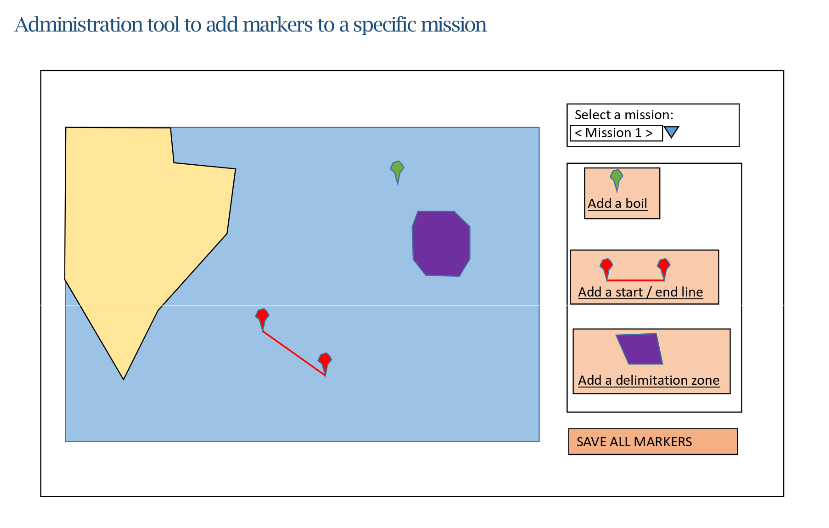
\includegraphics[width=15cm]{designedadminmarkers.png}
\caption{designed admin markers }
\label{fig-sample}
\end{figure}

\begin{figure}[h!]
\centering
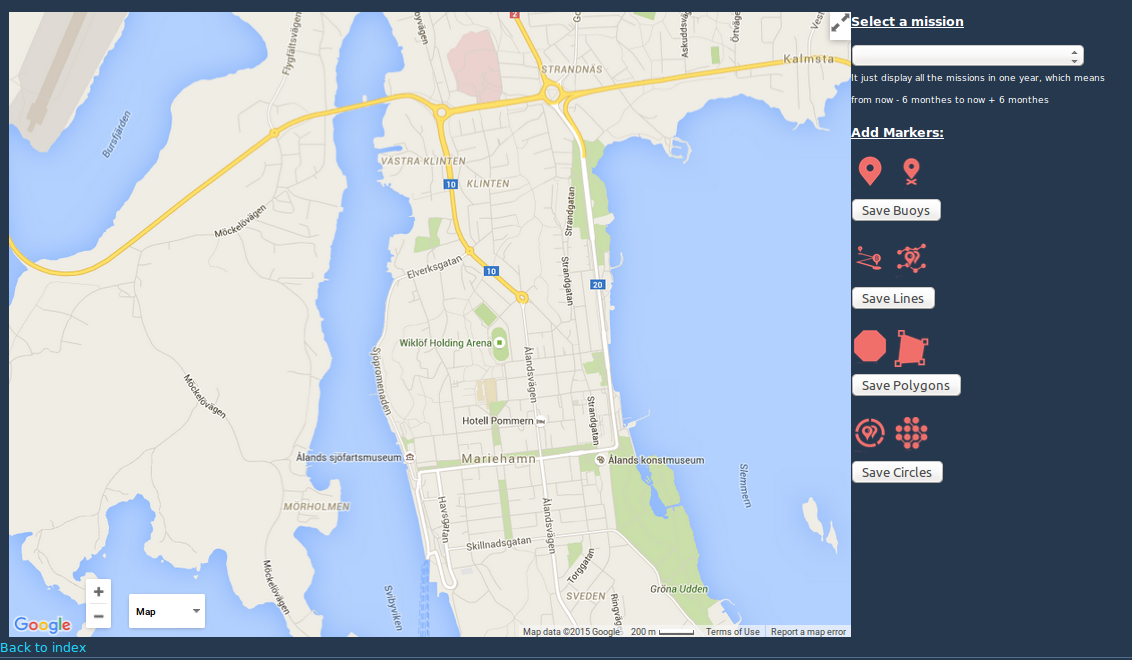
\includegraphics[width=15cm]{adminmarkers.png}
\caption{admin markers }
\label{fig-sample}
\end{figure}
The realization of creation of markers based on the Google map JavaScript APIs provided by Google company(https://developers.google.com/maps/documentation/javascript/markers). Actually, the JavaScript APIs provided the possibilities to add point, line, polygon and circle into the google map. And for each type markers, there are two possibilities to draw on the map: either draw the marker with the given coordinates, so then the marker is fixed on the map and can not be modified later, or draw the marker by clicking on the map directly, then it is up to the developer to add the options to drag or to move the marker or even change the size of marker dynamically. 
As a matter of fact, the last version could display some markers in the robots' path by using a gem called "gmaps4rails" which is easy to be applied into rails application, but since this gem also based on the Google map JavaScript API, in addition the gem changed and limited some options from Google APIs, so we could not use all the functions provided by Google API via the gem. In order to get more freedom, we had abandoned the gem, furthermore, the google API provided more customizable options(for example, we can change the icon of marker, add some animations for displaying the marker, the possibility to hide the marker instead of deleting the whole marker and also the adapt zoom for all the markers).
\begin{figure}[h!]
\centering
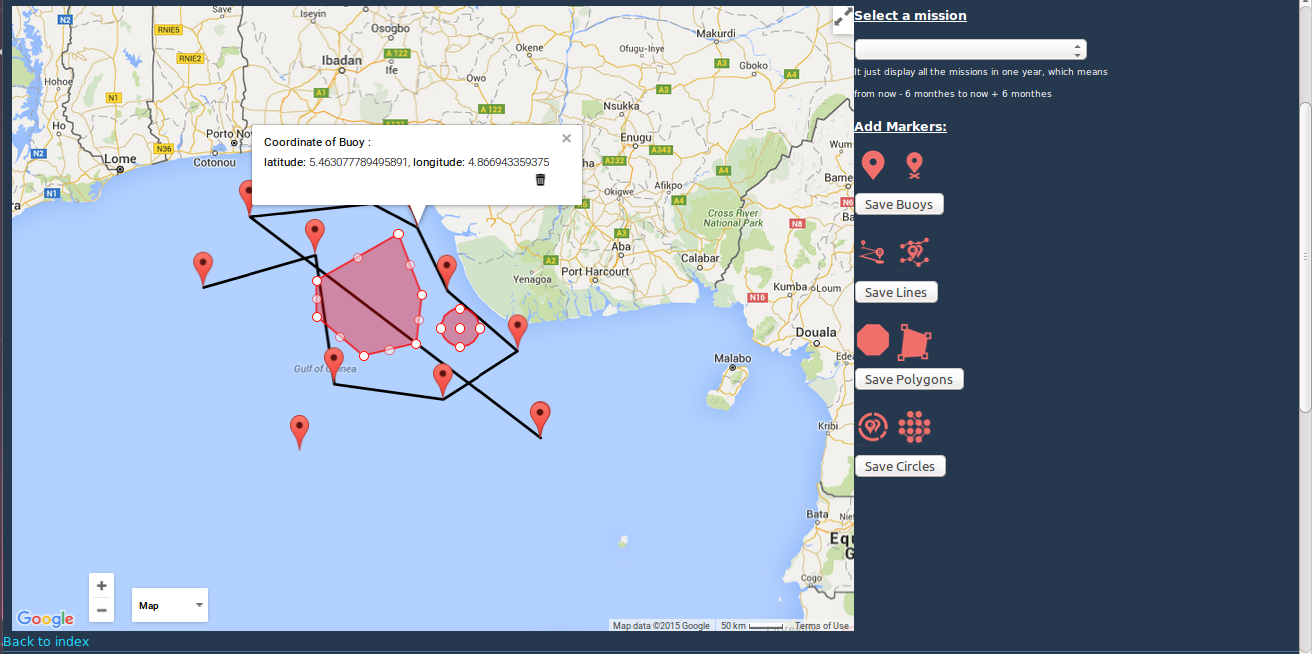
\includegraphics[width=15cm]{examplemarkers.png}
\caption{admin markers }
\label{fig-sample}
\end{figure}
\item{InfoWindow}
Moreover, Google map JavaScript API offers the possibilities to add some events to the marker or even some events for the mouse motion. Among all these options, what we are interested most is the possibility to display the infowindow for every marker to specify the accurate and precise coordinates of the robot's position. In fact, there are two ways to achieve the requirements.
\begin{itemize}
\item{Google API}
As a matter of fact, Google API provides the possibility to show the coordinate when clicking on the map directly, because google map capture the mouse action on the google map and then print the coordinates directly, but the limitation is that google map could only displays the coordinates of markers, if the user want to know much more information about the team(like: team name, the id of attempt and the tracker id), Google API could not meet all these demands. One advantage is that using google API do not need to communicate the server, so the response will be faster and it will reduce the pressure of server.
\begin{figure}[h!]
\centering
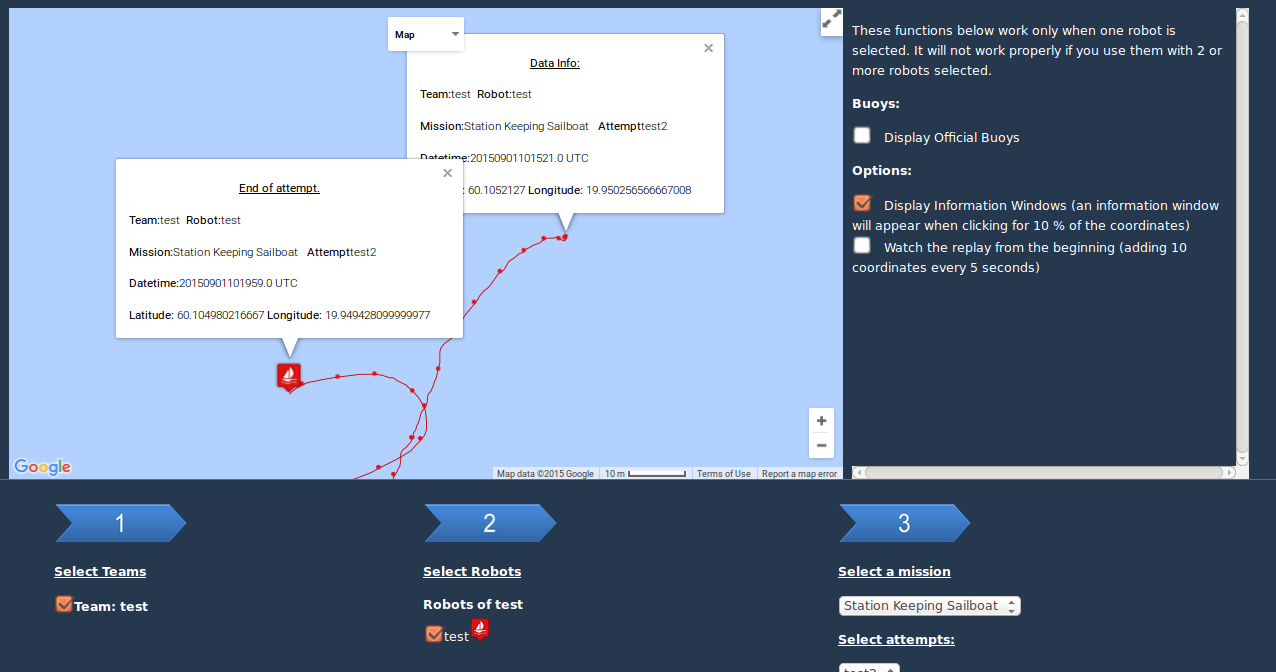
\includegraphics[width=15cm]{ajaxinfowindow.png}
\caption{admin markers }
\label{fig-sample}
\end{figure}
\item{Ajax request to communicate with server}
Obviously, communicating with server, we could get all the information we want, but the problem is that we need to send the Ajax requests, which will cost much more time, especially in most cases, there are hundreds and thousands data to display, even if the number of markers is 10 times less than the number of coordinates, we could imagine that 1000 positions need to display, then 1/10 of positions(which means 100) need to show the infowindow, also it means 100 Ajax requests, if every Ajax request lasts 30ms, then 100 Ajax requests last 3s, it means one user click a button one time, it will cost 3s to calculate for the server, when there are more than 10 users do the same things at the same time, the server would be broken absolutely.
\begin{figure}[h!]
\centering
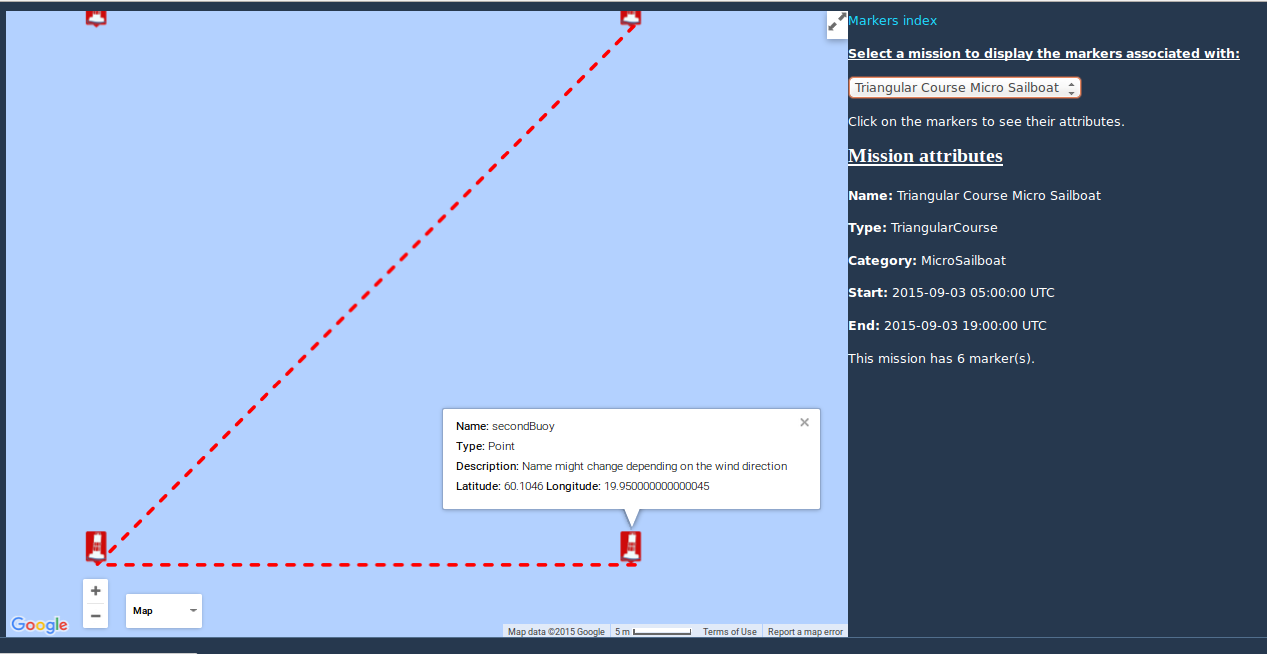
\includegraphics[width=15cm]{apiinfowindow.png}
\caption{admin markers }
\label{fig-sample}
\end{figure}
\end{itemize}
So actually, there is not any better way to do it, the different method meets different requirements, finally we had mixed these two ways to achieve our target.
\end{itemize}